\documentclass[a4paper]{article}
\usepackage{tikz}
\usetikzlibrary{calc,positioning,arrows}
\usepackage[a4paper]{geometry}
\usepackage[sfdefault,book]{FiraSans}

\begin{document}
\thispagestyle{empty}

\begin{tikzpicture}[remember picture,overlay, scale=1
    , every node/.style={node distance=1mm} ]

    \node[opacity=0.9,inner sep=0pt] (background) at (current page.center)
    {
        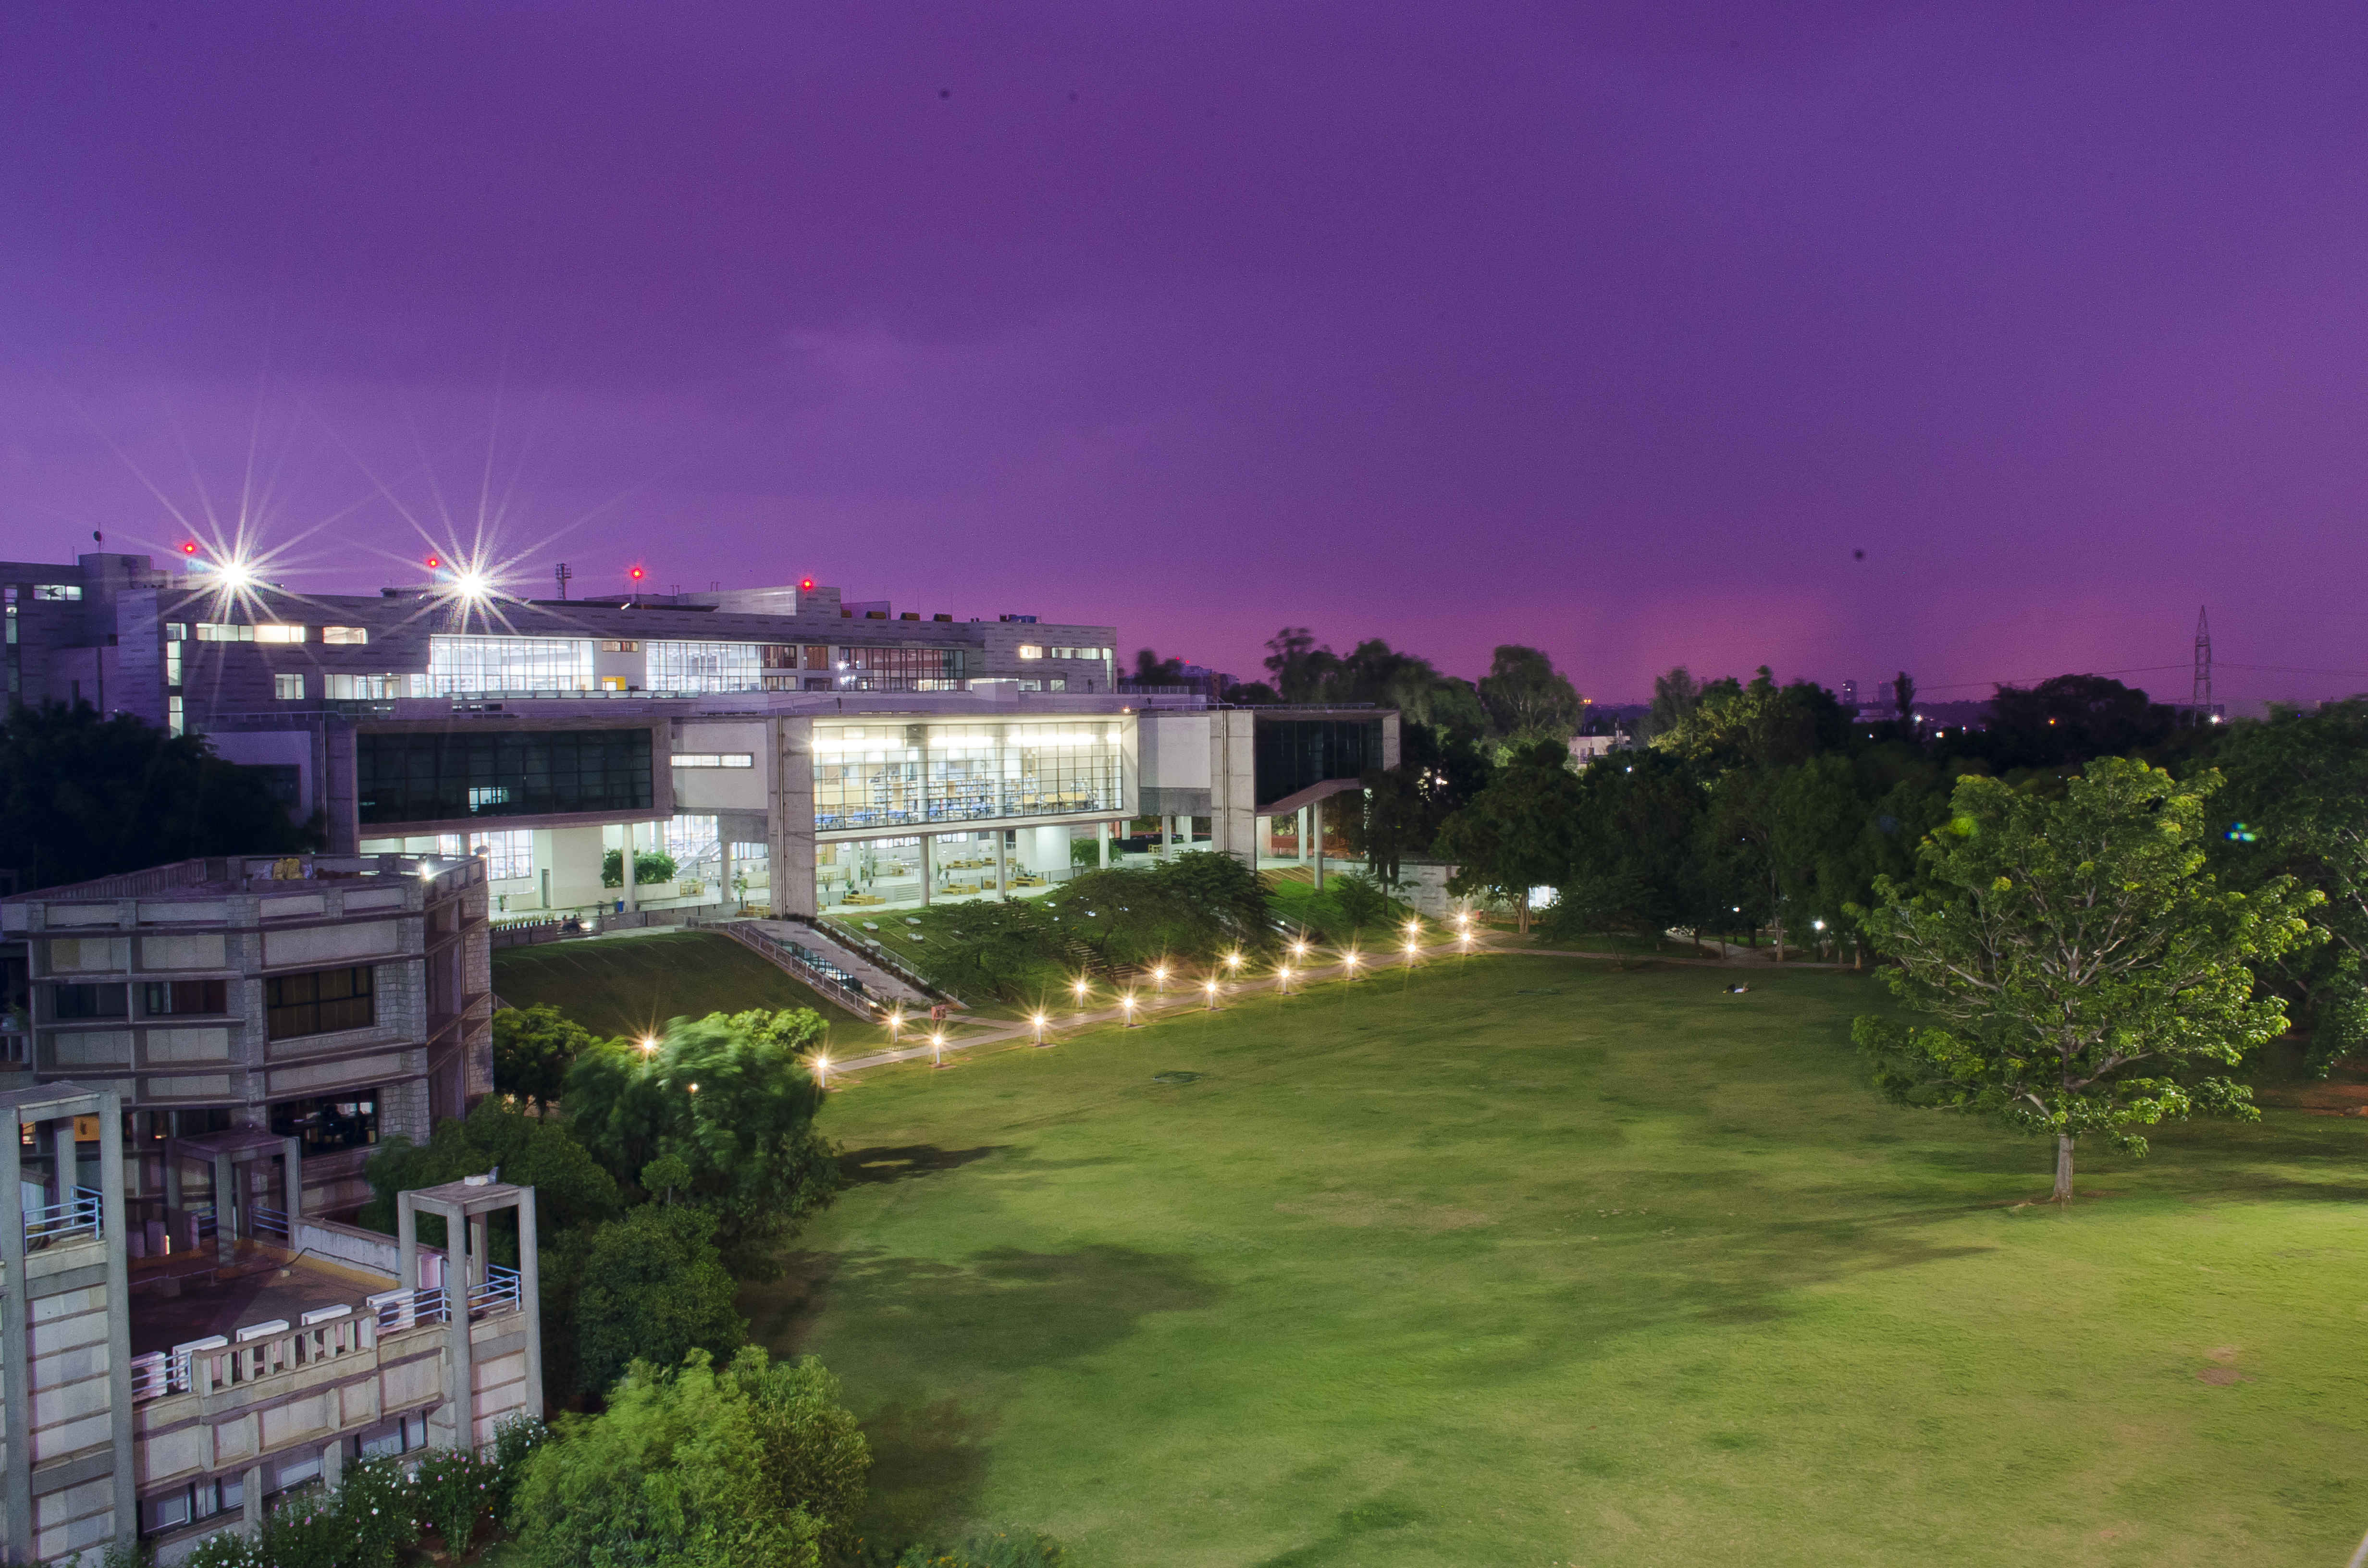
\includegraphics[
            %width=\paperwidth,
            %height=\paperheight]{./images/background_low_res.jpg}
            height=\paperheight]{./images/background_low_res_cricket.jpg}
    };

    \edef\cl{white}
    \node[text width=0.6\paperwidth] (title) at (0.45\paperwidth,0) { 
        \textcolor{\cl}{\fontsize{1.5cm}{2cm}\selectfont \hfill Student Handbook}
    };

    \node[text width=0.6\paperwidth, below=of title ] (ncbs) {
        \textcolor{\cl}{\raggedleft \hfill \Huge 2017}
    };

    % Logos
    \node[] (ncbs) at (0.55\paperwidth,-0.8\paperheight) { 
        
\includegraphics[height=2cm]{../Logos/ncbs_logo.png}
    };
    \node[] (ncbs) at (0.05\paperwidth,-0.8\paperheight) { 
        
\includegraphics[height=2cm]{../Logos/inStem_logo.png}
    };
    
    % credit
    \node[inner sep=2pt,yshift=2mm,xshift=3cm] (credit) 
        at (current page.south west) {
            \small \tt Image credit : Unknown
        };

\end{tikzpicture}    


\end{document}
